\documentclass[10pt]{beamer}
%
% Choose how your presentation looks.
%
% For more themes, color themes and font themes, see:
% http://deic.uab.es/~iblanes/beamer_gallery/index_by_theme.htmhttps://www.overleaf.com/10032604zwwjvhdnkfcz#l
%
\mode<presentation>
{
  \usetheme{Boadilla}    % or try Darmstadt, Madrid, Warsaw, ...
  \usecolortheme{crane}  % or try albatross, beaver, crane, ...
  \usefonttheme{default} % or try serif, structurebold, ...
  \setbeamertemplate{navigation symbols}{}
  \setbeamertemplate{caption}[numbered]
} 

% \usepackage[english]{babel}
\usepackage[utf8x]{inputenc}
% \usepackage{listings}
% \usepackage{graphicx}
\usepackage{textpos}  % for putting logo
\usepackage{color}    % for setting font color
% \usepackage{hyperref} % for url
\usepackage{tikz}     % transparent background image
% \usepackage{eurosym}  % euro sign
% \usepackage{multirow} %
% \usepackage{appendixnumberbeamer} % count presentation slides only
% \usepackage{pbox} % new line in cell of table
% \usepackage{booktabs} % toprule and bottomrule

% Change the color of theme
%\definecolor{OU Crimson}{RGB}{153,0,0}% See http://en.wikipedia.org/wiki/Shades_of_red
\definecolor{Oklahoma_Sooners}{RGB}{126,4,3}
\setbeamercolor{title}{fg=white,bg=Oklahoma_Sooners}
\setbeamercolor{frametitle}{fg=white,bg=Oklahoma_Sooners}
\setbeamercolor{author in head/foot}{fg=white,bg=Oklahoma_Sooners}
\setbeamercolor{title in head/foot}{fg=white,bg=Oklahoma_Sooners}
\setbeamercolor{date in head/foot}{fg=white,bg=Oklahoma_Sooners}
\setbeamercolor{block title}{fg=white,bg=Oklahoma_Sooners}

% Put the OU logo in the top right corner
\addtobeamertemplate{frametitle}{}{%
  \begin{textblock*}{100mm}(.95\textwidth,-0.88cm)
    
\includegraphics[height=0.8cm,width=1.04cm]{figures/Oklahoma_Sooners}
  \end{textblock*}
}


\title[PhD Defense]{Search for Supersymmetry}
\subtitle{Search for electroweak production of supersymmetric states in Non-Universal Higgs Mass model with two extra parameters compressed scenario with the ATLAS detector}
\author[Yu-Ting]{Yu-Ting Shen}
\institute[OU]{Department of Physics and Astronomy\\The University of Oklahoma}
% \date{\today}
\date{April 17, 2018}



\begin{document}

\begin{frame}
    \titlepage
\end{frame}

% Uncomment these lines for an automatically generated outline.
%\begin{frame}{Outline}
%  \tableofcontents
%\end{frame}

%\usebackgroundtemplate{\tikz\node[opacity=0.3]\includegraphics[height=\paperheight]{ATLAS-Logo-Square-Blue-RGB.png}}

\section{Particle physics overview}
% \frame{\sectionpage}

{
\usebackgroundtemplate{%
    \tikz\node[opacity=0.2]{
        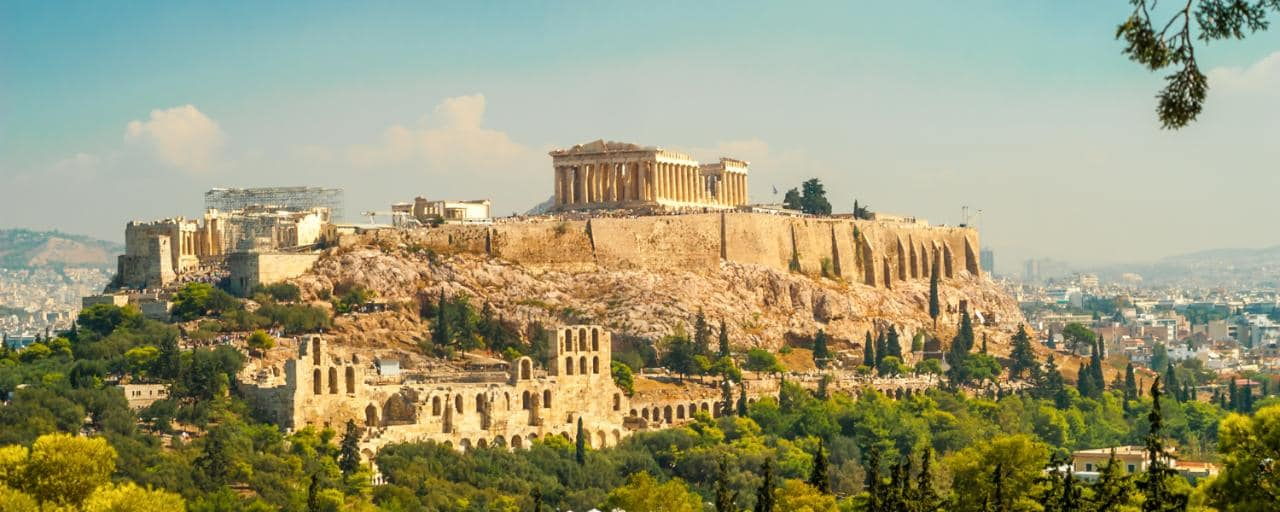
\includegraphics[height=\paperheight]{figures/ancient_greece.jpg}
    };
}

\begin{frame}{History}
    \begin{center}
        \Huge{Ancient Greece...}
    \end{center}
\end{frame}

\begin{frame}{History}
    \begin{columns}
        \begin{column}{0.8\textwidth}
            \begin{itemize}
                \item Aristotle:
                \begin{itemize}
                    \item All materials on Earth were made of the four elements: Earth, Fire, Water, and Air
                    \item All substances were made of small amounts of these four elements of matter
                \end{itemize}
                \item 460 - 370 B.C. Democritus:
                \begin{itemize}
                    \item All matter consists of invisible particles called atoms
                    \item Atoms are indestructible
                    \item Atoms are solid but invisible
                    \item Atoms are homogenous
                    \item Atoms differ in size, shape, mass, position, and arrangement
                    \begin{itemize}
                        \item Solids are made of small, pointy atoms
                        \item Liquids are made of large, round atoms
                        \item Oils are made of very fine, small atoms that can easily slip past each other
                    \end{itemize}
                \end{itemize}
            \end{itemize}
        \end{column}
        \begin{column}{0.16\textwidth}
            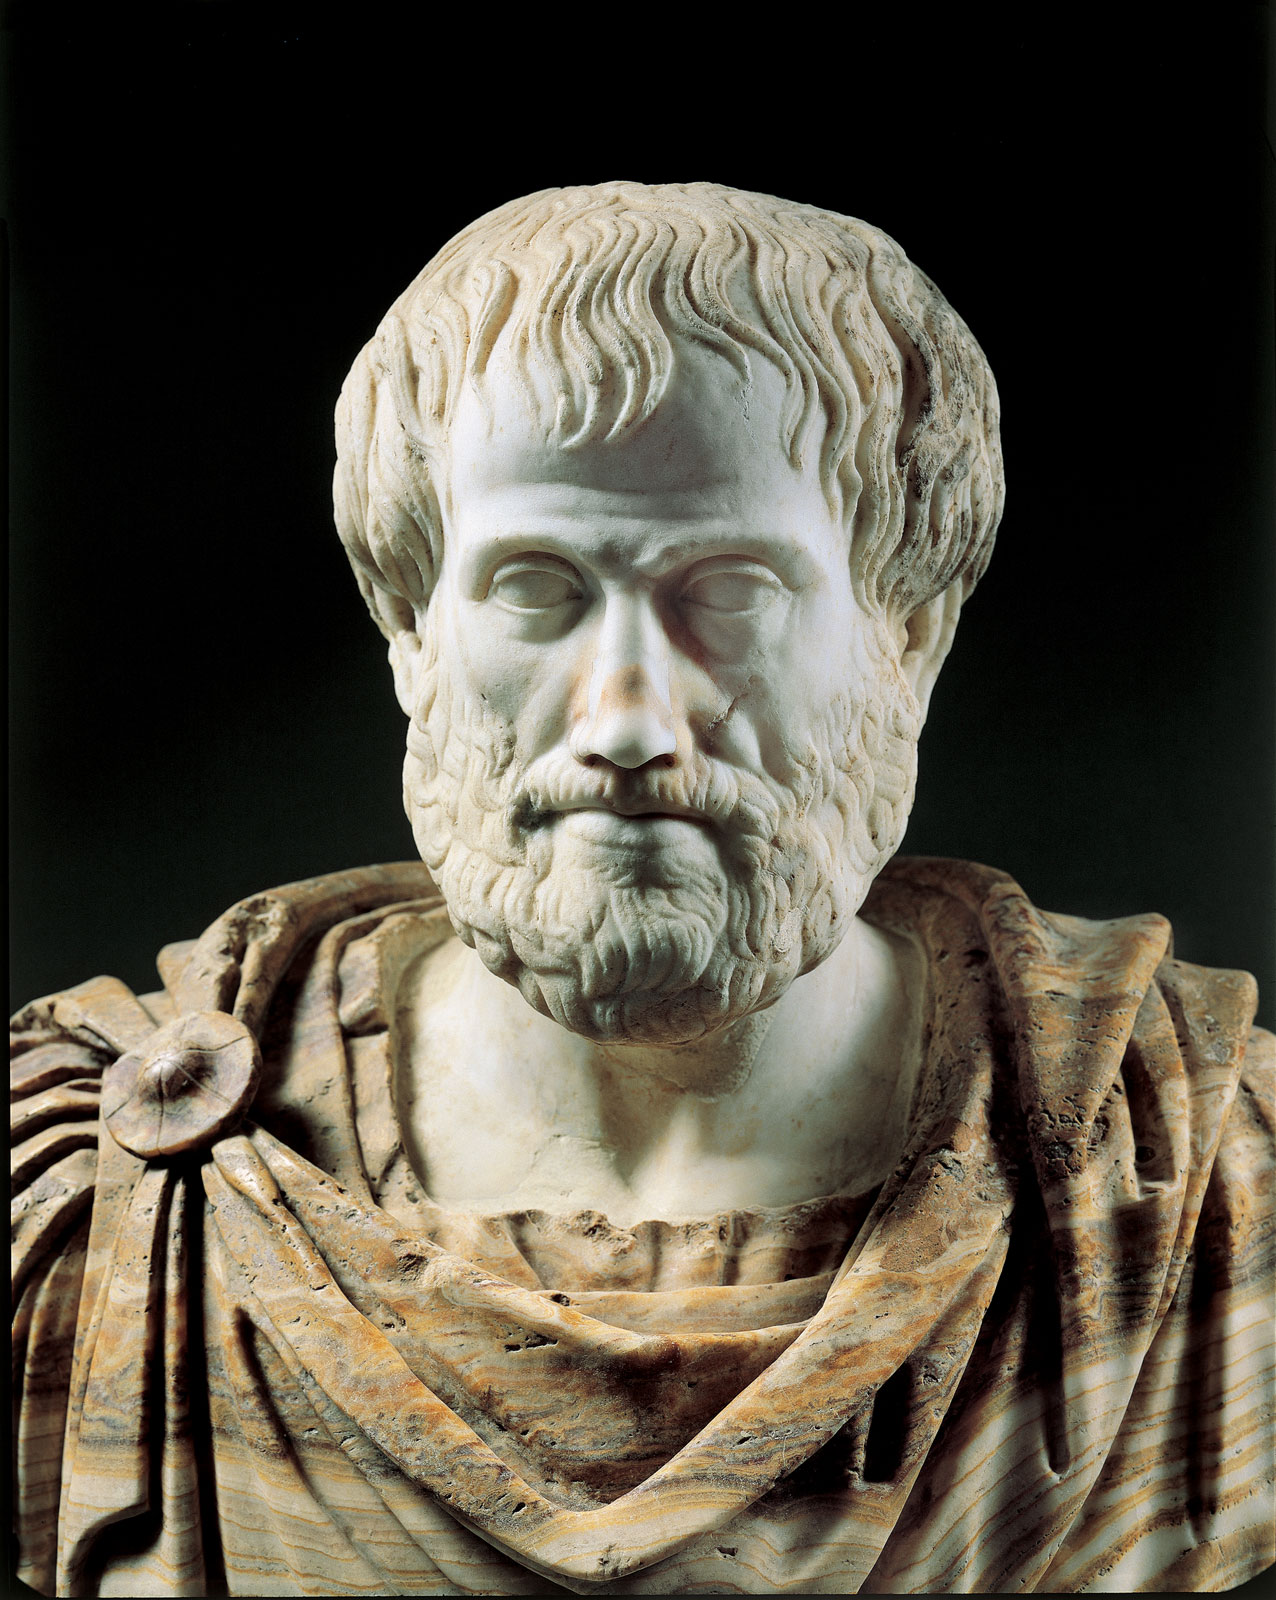
\includegraphics[scale=0.05]{figures/Aristotle.jpg}\\
            \includegraphics[scale=0.117]{figures/democritus.png}
        \end{column}
    \end{columns}
\end{frame}
}

{
\usebackgroundtemplate{%
    \tikz\node[opacity=0.2]{
        
\includegraphics[height=\paperheight]{figures/20_century.png}
    };
}

\begin{frame}{History}
    \begin{center}
        \Huge{20 Century...}
    \end{center}
\end{frame}

\begin{frame}{History}
    \begin{itemize}
        \item 1803 John Dalton:
            \begin{itemize}
                \item Elements are made of extremely small particles called atoms
                \item Atoms cannot be subdivided, created or destroyed
            \end{itemize}
        % \item R\"{o}ntgen discovered $X$-rays in 1895
        \item J.J Thomson discovered electrons and proposed the Plum pudding model in 1904
        \item Rutherford discovered subatomic structure in 1909: nucleus
        \item Chadwick discovered the neutron in 1932
        \item Gell-Mann and Zweig proposed quark model in 1964 and quarks were observed in 1968.
    \end{itemize}
    \begin{figure}
        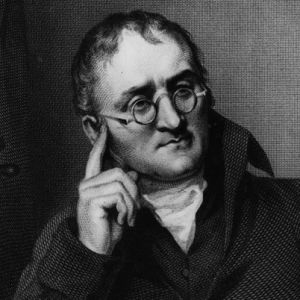
\includegraphics[height=0.25\textheight]{figures/Dalton.jpg}
        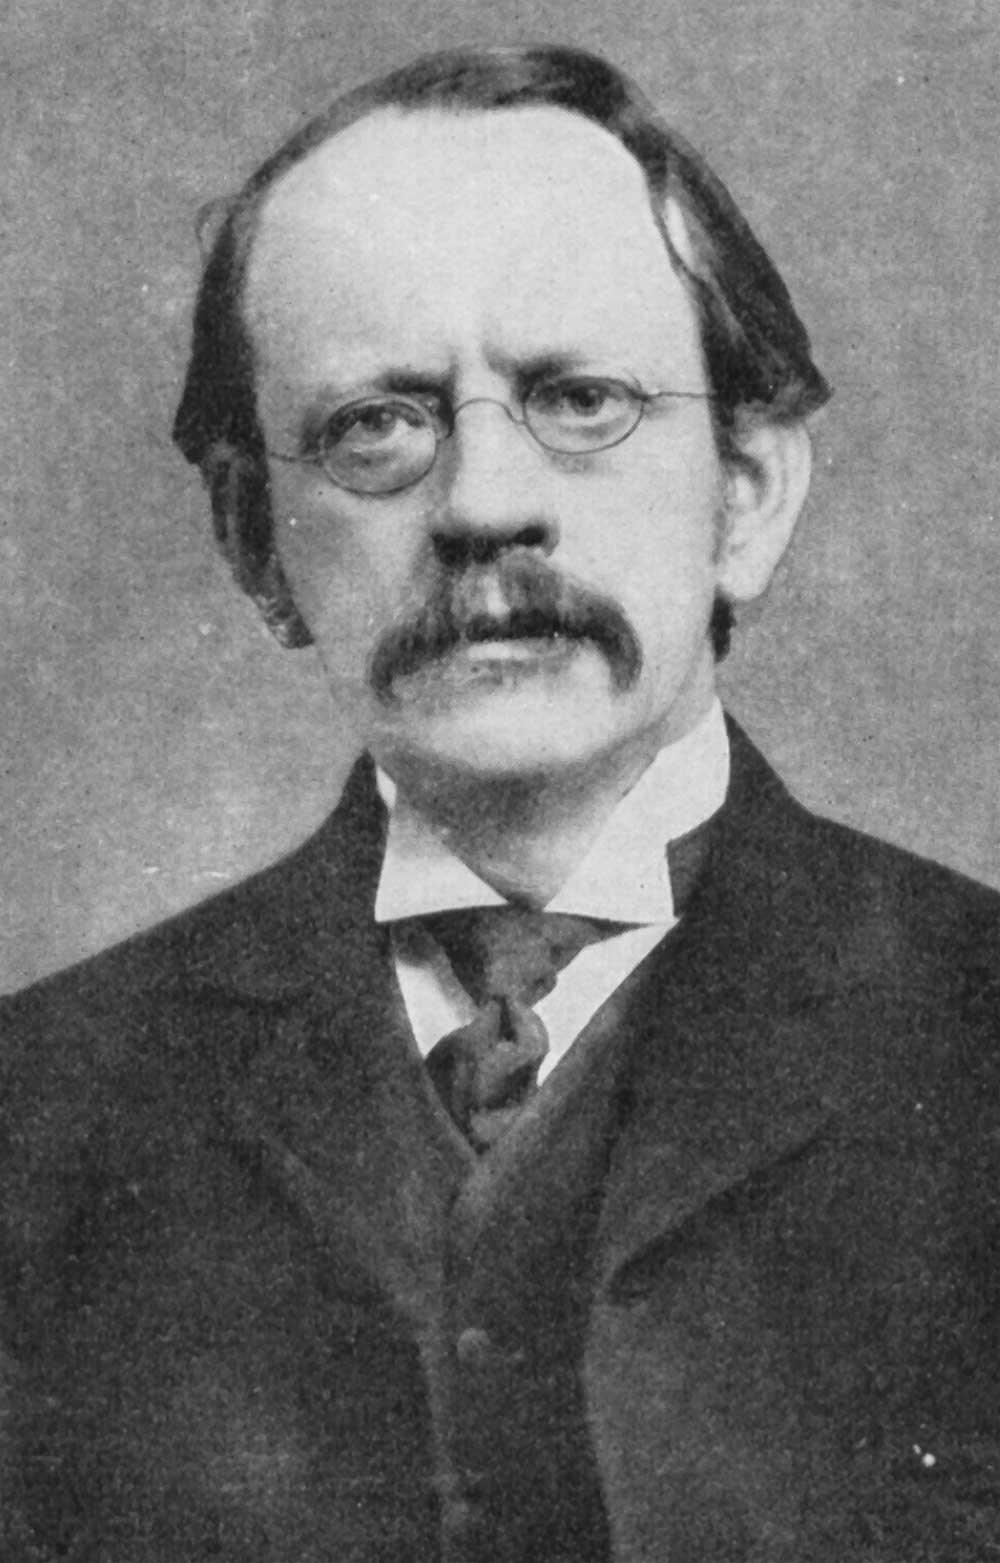
\includegraphics[height=0.25\textheight]{figures/Thomson.jpg}
        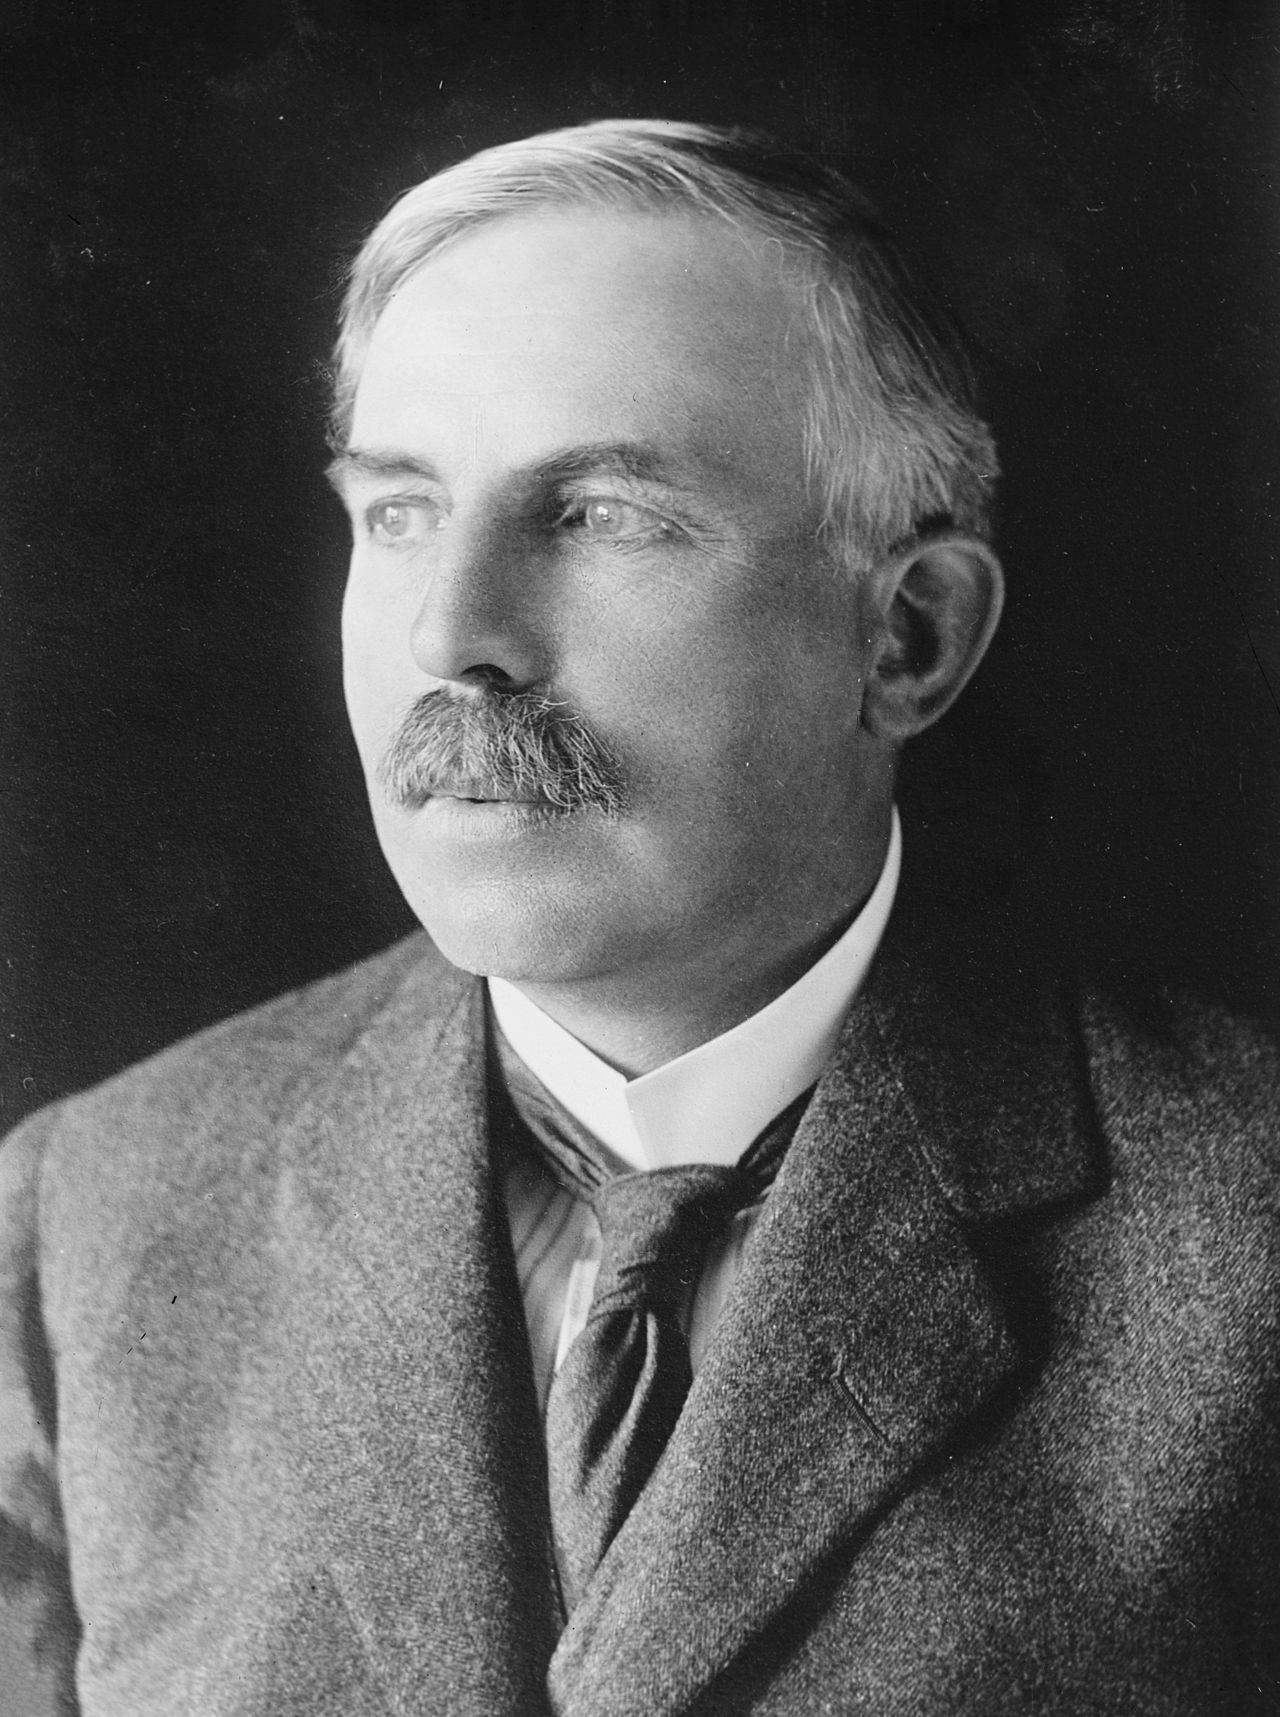
\includegraphics[height=0.25\textheight]{figures/Rutherford.jpg}
        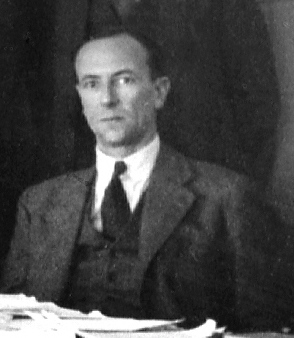
\includegraphics[height=0.25\textheight]{figures/Chadwick.jpg}
        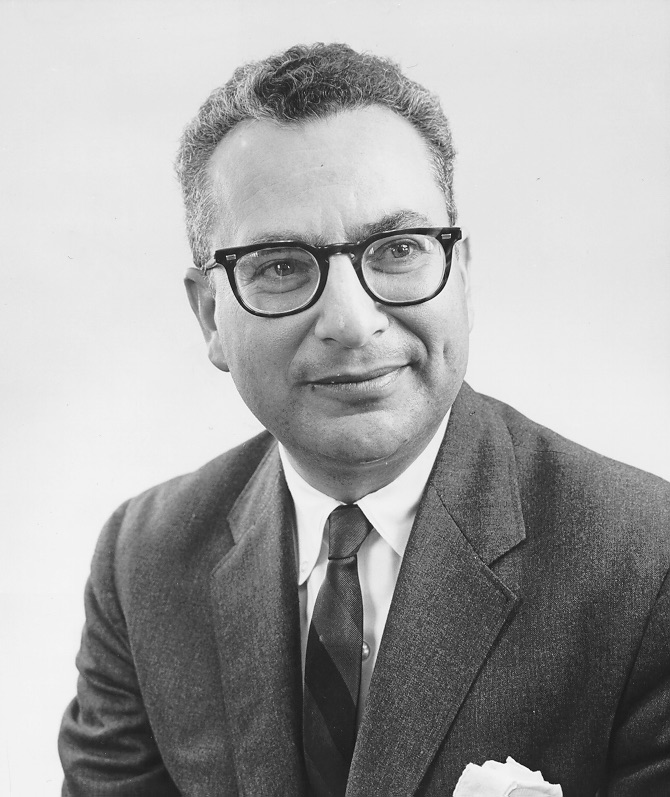
\includegraphics[height=0.25\textheight]{figures/Gell-Mann.jpg}
        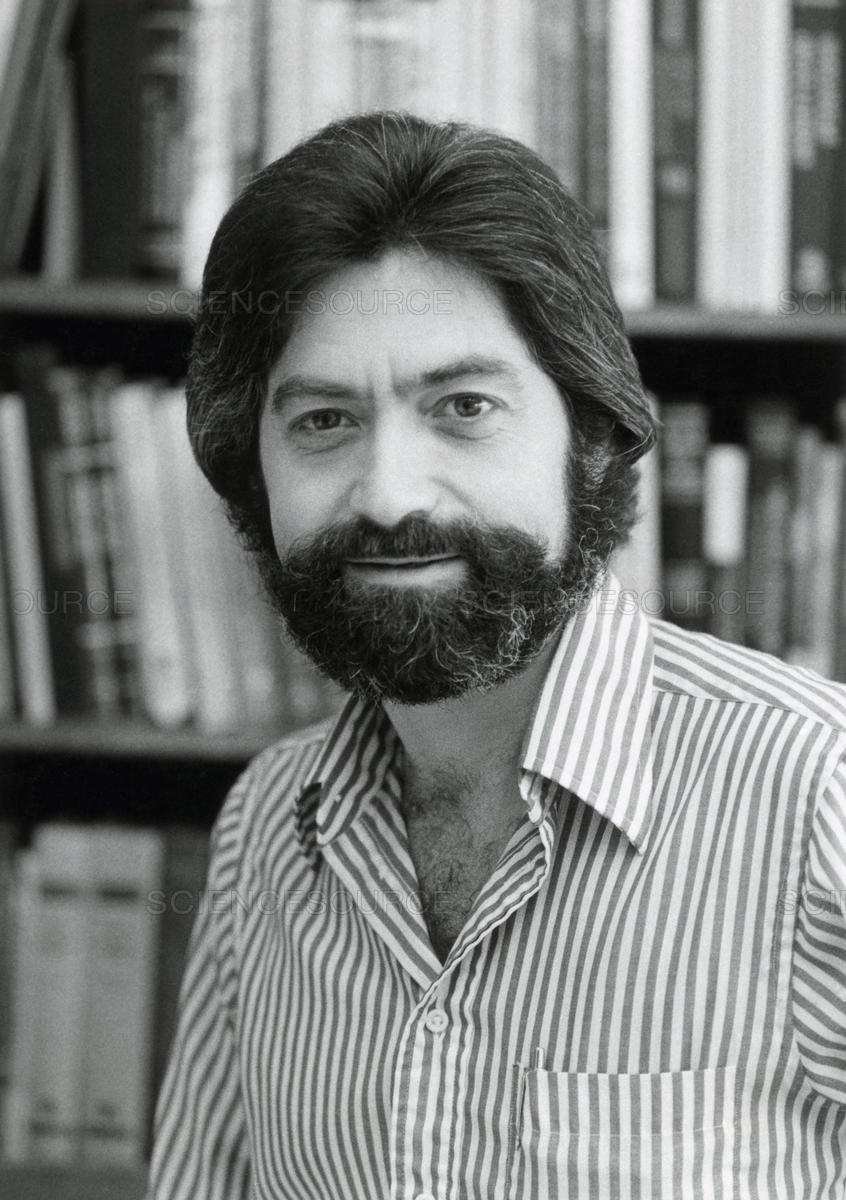
\includegraphics[height=0.25\textheight]{figures/Zweig.jpg}
    \end{figure}
\end{frame}
}

\begin{frame}{History}
    \begin{columns}
        \begin{column}{0.8\textwidth}
            \begin{itemize}
            \item Plum pudding model
            \begin{itemize}
                \item Proposed by J.J Thomson
                \item Atoms are electrically neutral $\Rightarrow$  There must be a positive charge as well.
                \item An atom is consisted of negative electrons randomly scattered within a sphere of positive charge.
            \end{itemize}
            \item Rutherford model
            \begin{itemize}
                \item Proposed by Rutherford based on the experimental results.
                \item An atom is made up of a central charge (atomic nucleus) surrounded by a cloud of (presumably) orbiting electrons. I
                \item Nucleus is a very small volumn in comparison to the rest of the atom. A relatively high central charge concentrated in nucleus and it also contains the bulk of the atomic mass of the atom.
            \end{itemize}
            \item Bohr model
            \begin{itemize}
                \item Proposed by Bohr
                \item The atom is a small, positively charged nucleus surrounded by electrons that travel in circular orbits around the nucleus 
                \item It is similar to structure of the Solar System.
            \end{itemize}
        \end{itemize}
        \end{column}
        \begin{column}{0.2\textwidth}
            \begin{figure}
                
\includegraphics[height=0.25\textheight]{figures/Plum_pudding_model.png}\\
                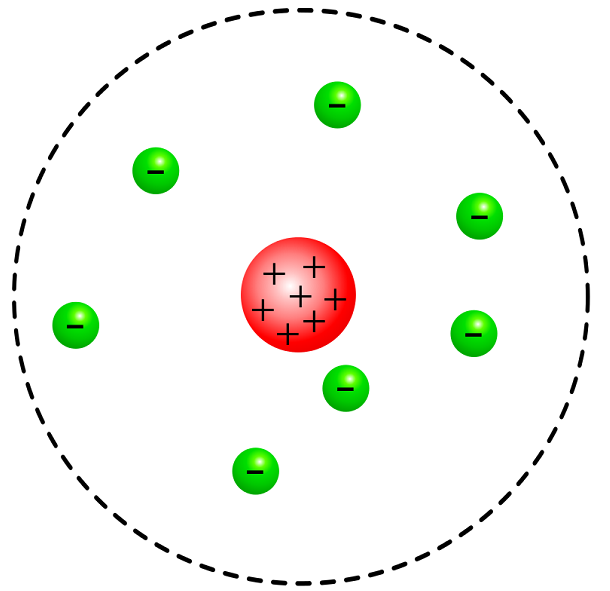
\includegraphics[height=0.25\textheight]{figures/Rutherford_model.png}\\
                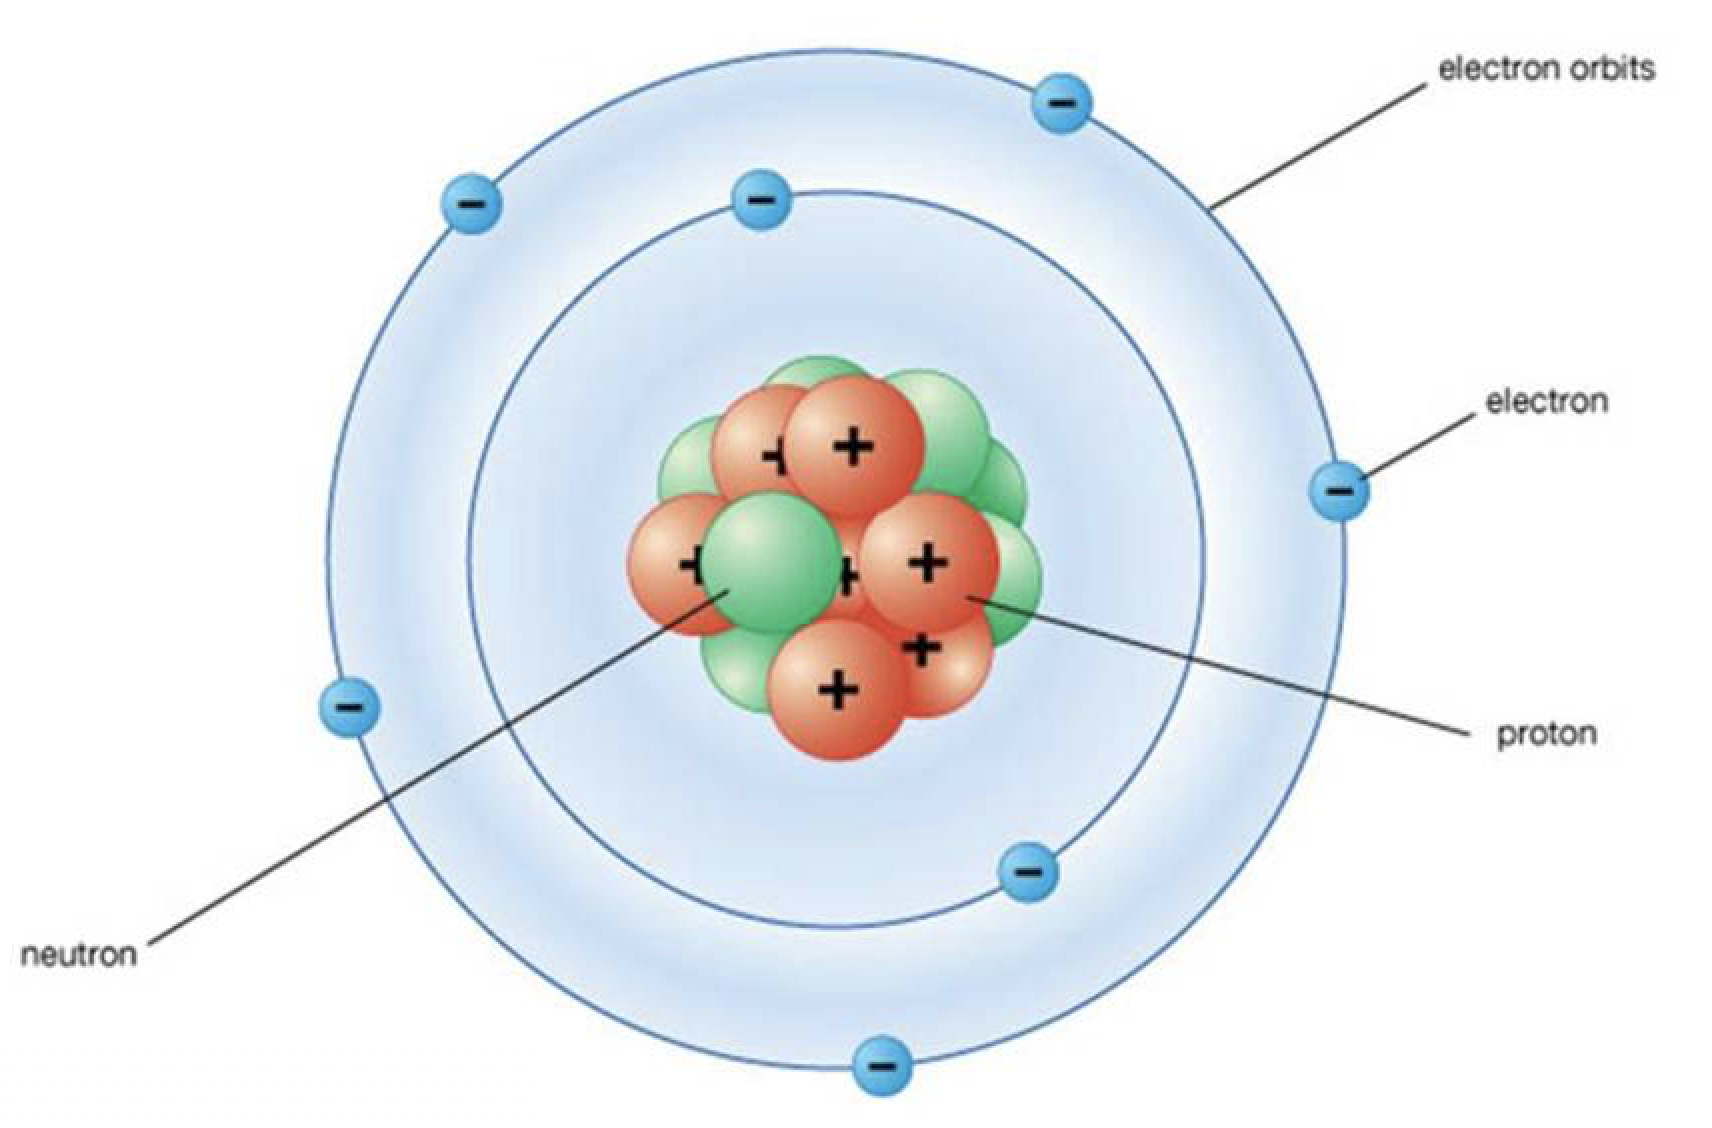
\includegraphics[height=0.18\textheight]{figures/Bohr_model.png}
            \end{figure}
        \end{column}
    \end{columns}
\end{frame}

\begin{frame}{History}
    \begin{itemize}
        \item The atomic structure we know now:
    \end{itemize}
    \begin{figure}
        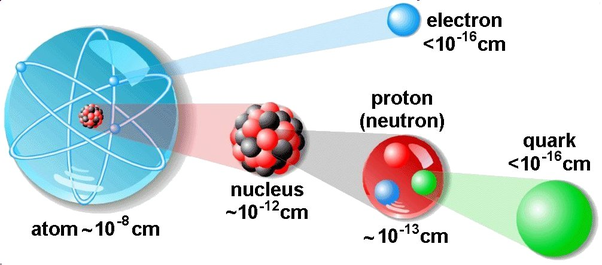
\includegraphics[scale=0.5]{figures/atom_structure.png}
    \end{figure}
\end{frame}

\begin{frame}{Standard Model of Particle Physics}
    \begin{itemize}
        \item Particle Physics
        \begin{itemize}
            \item Also called high energy physics
            \item Studies the nature of the particles and the fundamental interactions
        \end{itemize}
        \item Standard Model
        \begin{itemize}
            \item The Standard Model of particle physics describes current understanding of fundamental particles and their interactions
        \end{itemize}
    \end{itemize}
\end{frame}

\begin{frame}{Standard Model of Particle Physics}
    \begin{columns}
        \begin{column}{0.4\textwidth}
            \begin{itemize}
                \item 3 principles
                \begin{itemize}
                    \item Special Relativity
                    \item Quantum Mechanics
                    \item Gauge Invariance:\\$SU(3) \otimes SU(2) \otimes U(1)$
                \end{itemize}
                \item 2 catogeries
                \begin{itemize}
                    \item Ferminos: spin 1/2\\matter particles
                    \item Bosons: integer spin\\force carriers
                \end{itemize}
                \item Higgs boson
                \begin{itemize}
                    \item Discovered in 2012
                    \item Gives mass to fundamental particles
                    \item Spontaneous symmetry breaking
                \end{itemize}
            \end{itemize}
        \end{column}
        \begin{column}{0.6\textwidth}
            \begin{figure}
                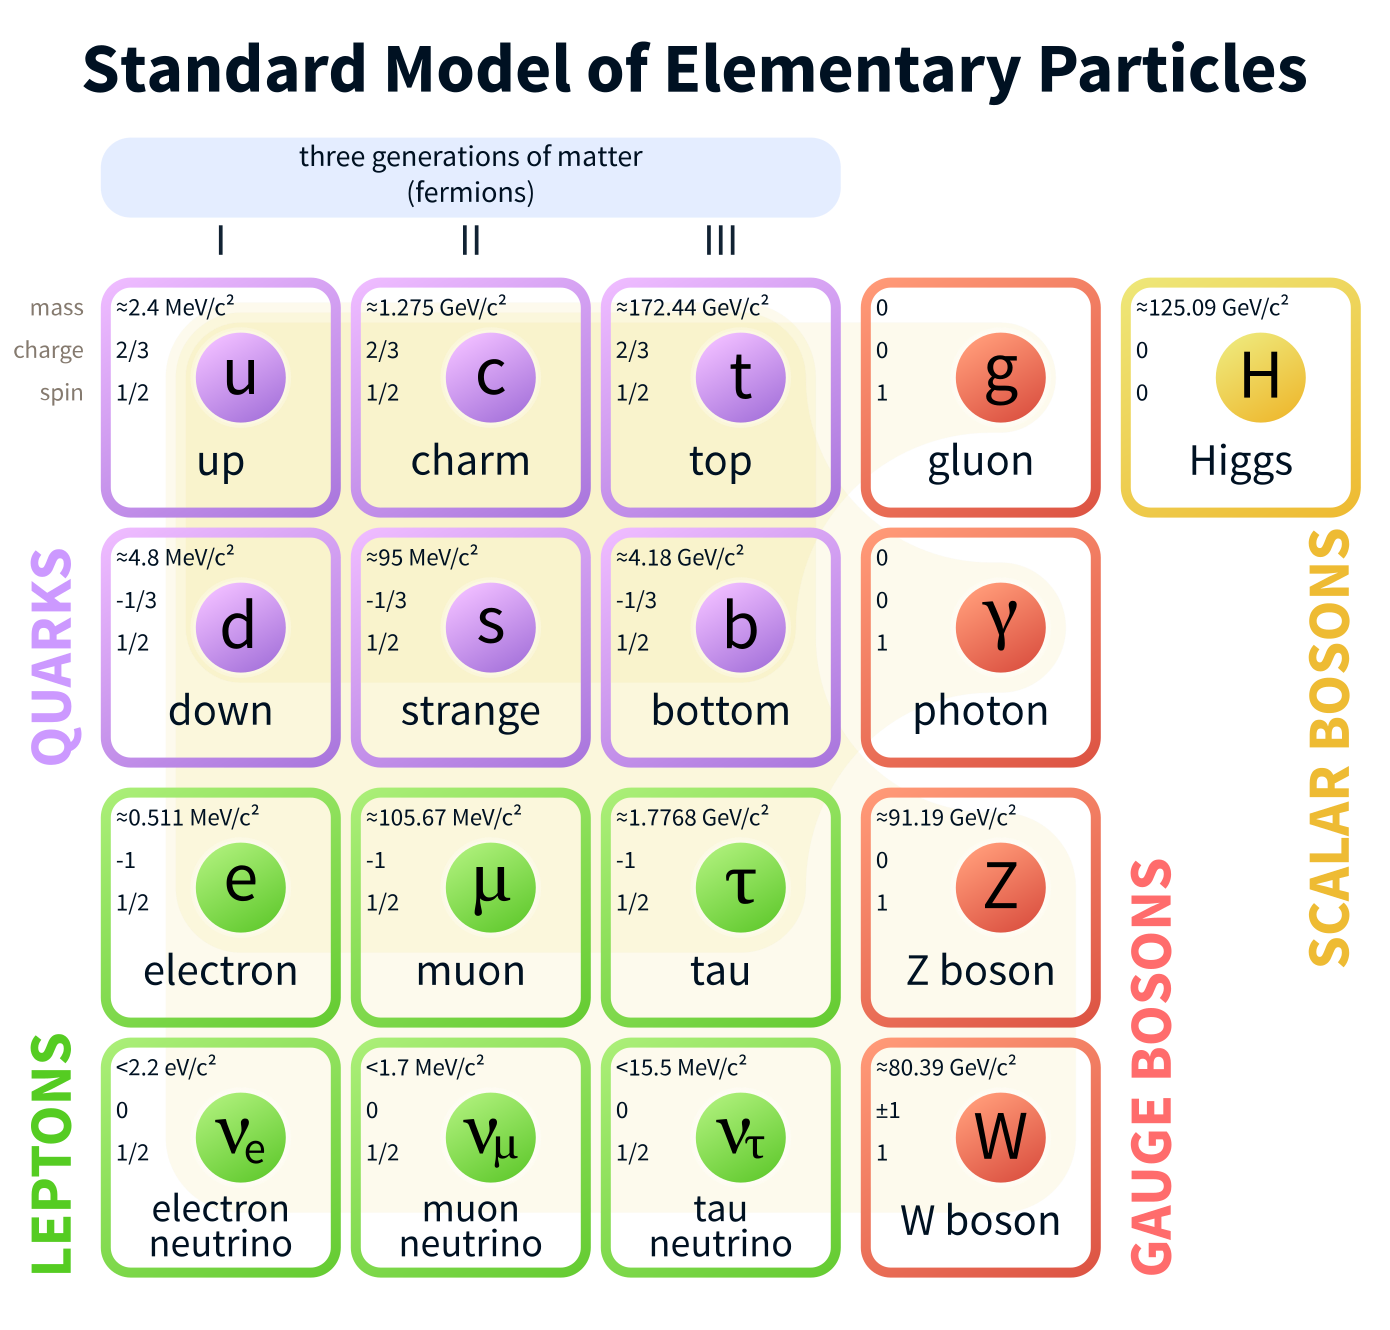
\includegraphics[scale=0.14]{figures/Standard_Model_of_Elementary_Particles.png}
            \end{figure}
        \end{column}
    \end{columns}
\end{frame}

\begin{frame}{Standard Model of Particle Physics}
    \begin{figure}
        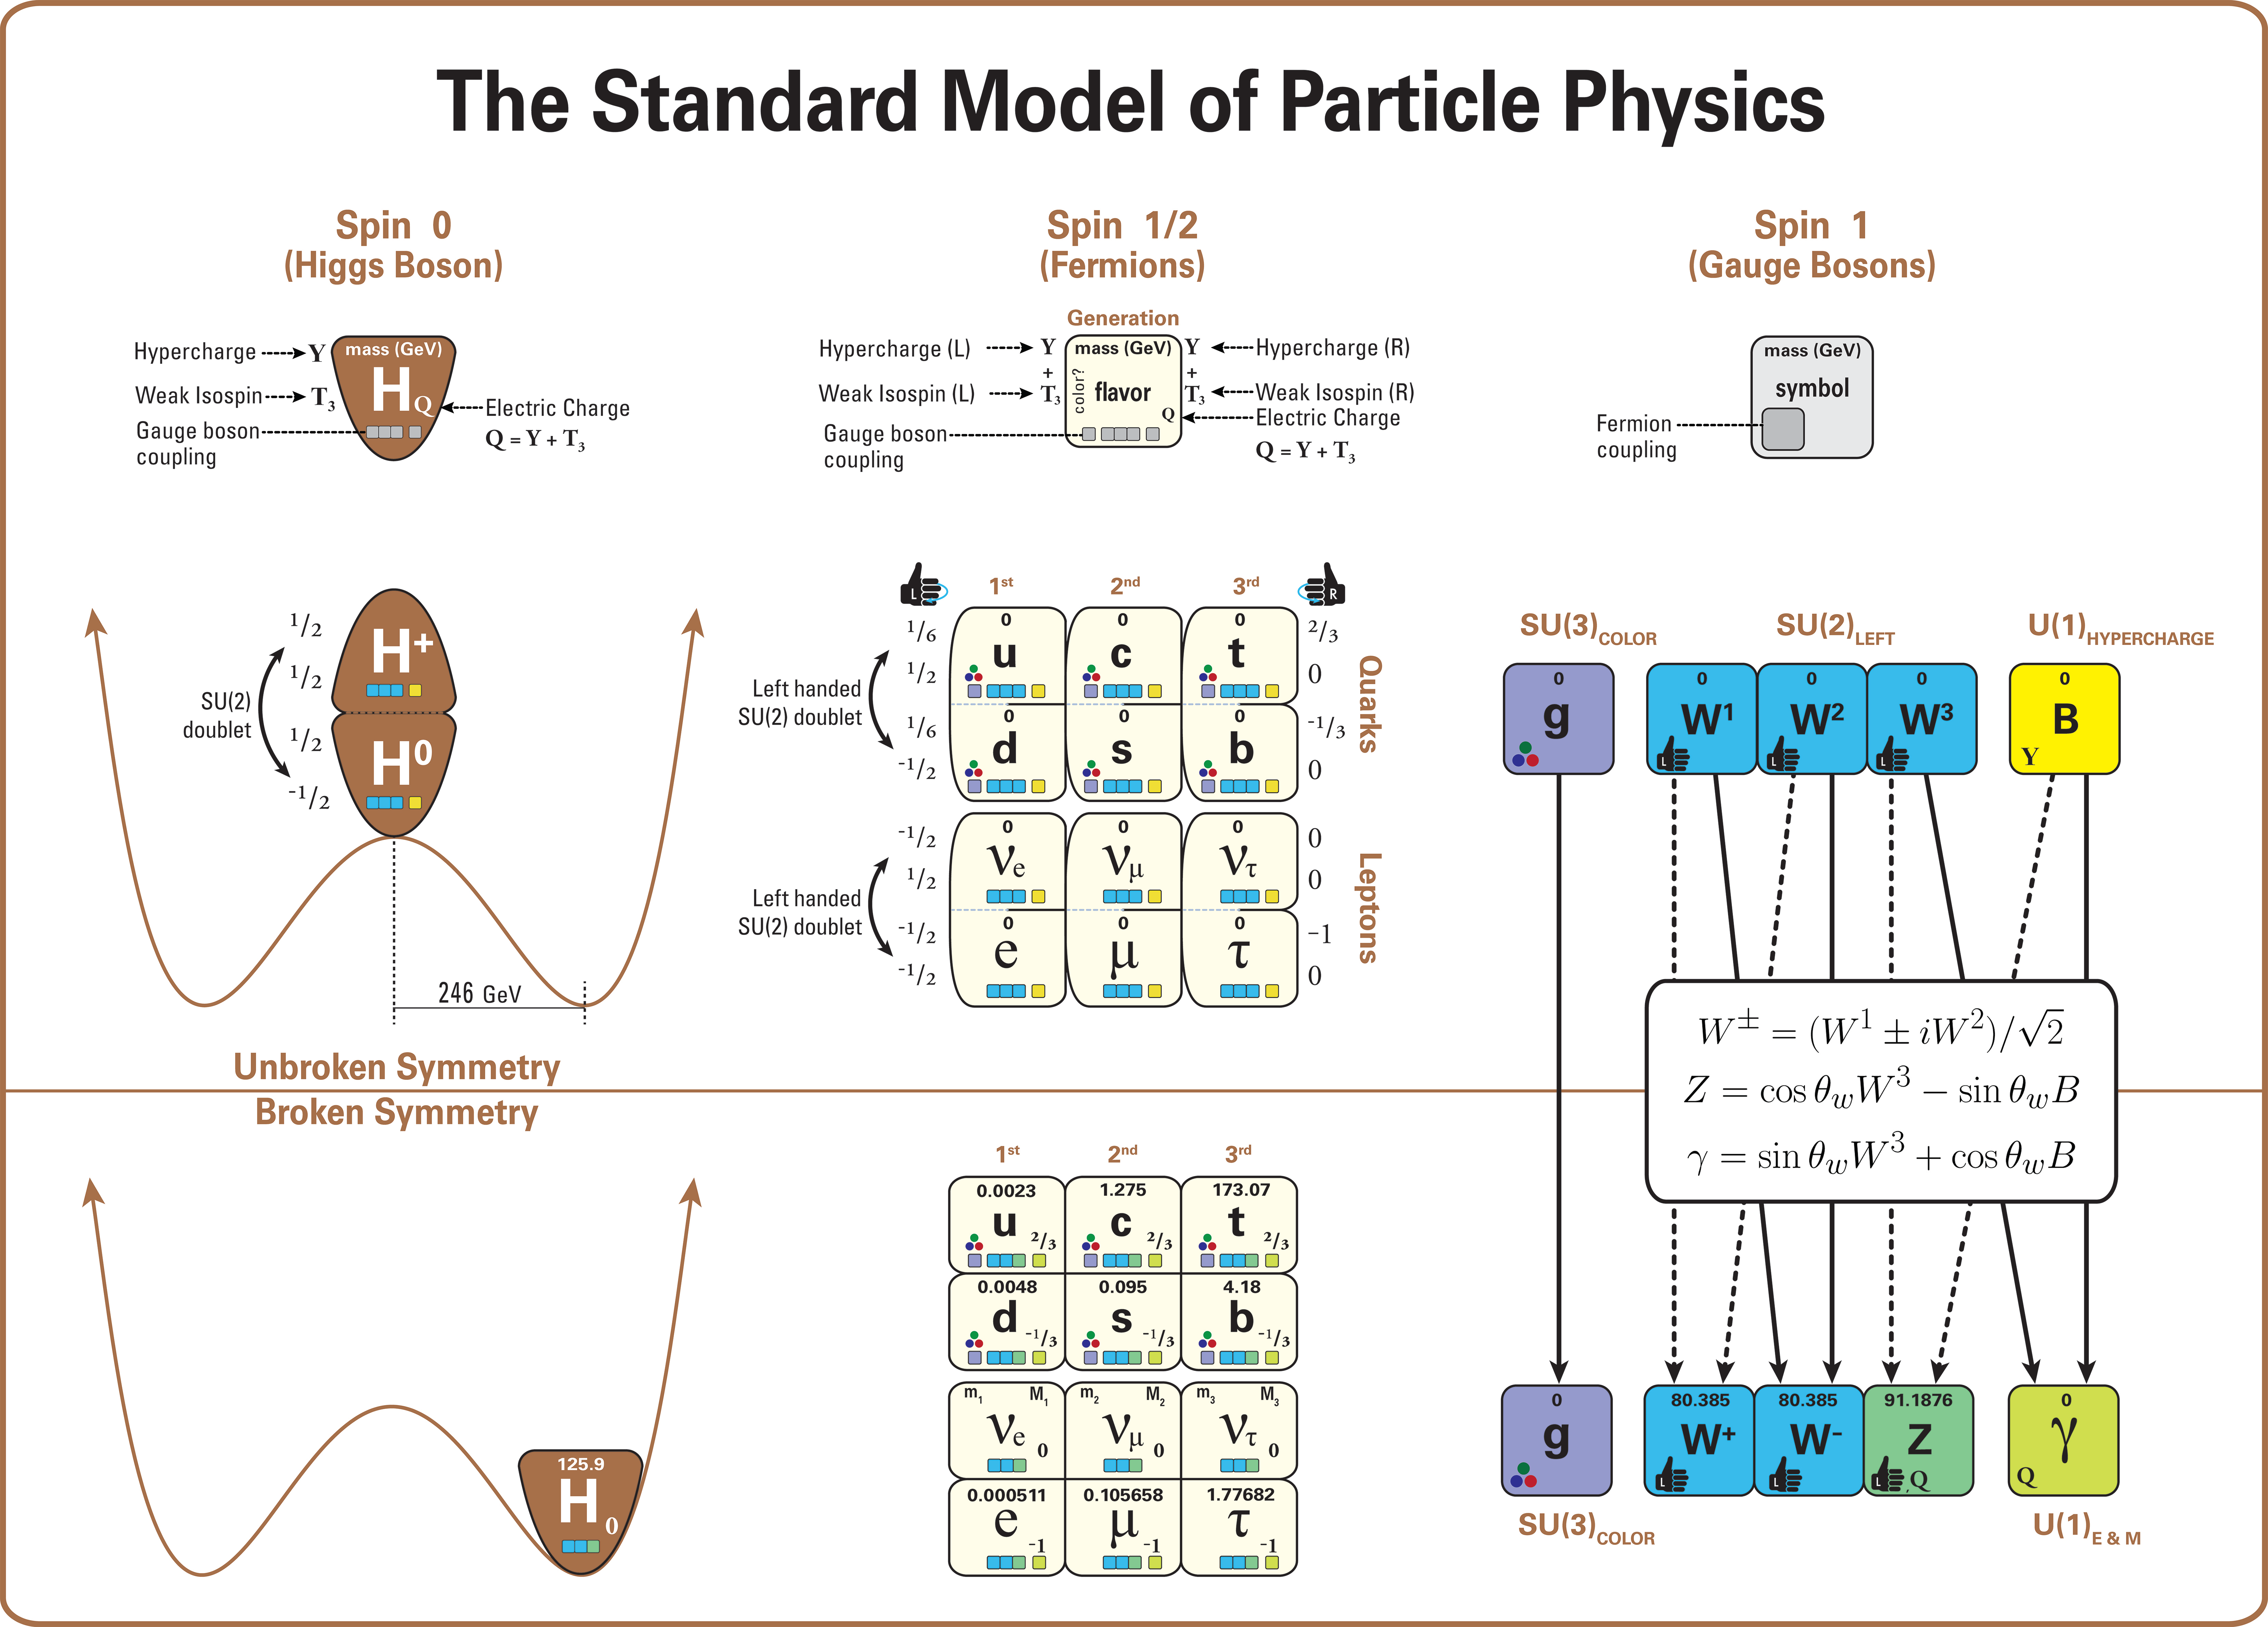
\includegraphics[width=0.9\textwidth]{figures/Standard_Model_Of_Particle_Physics--Most_Complete_Diagram.png}
    \end{figure}
\end{frame}

\begin{frame}{Open questions of the SM}
    \begin{itemize}
        \item The SM cannot explain: hierarchy problem, the Dark Matter \& Dark Energy, Grand unification, etc..
        \item Example: Dark Matter \& Dark Energy
        \begin{itemize}
            \item Dark Matter doesn't absort, emit, and relect light
            \item Dark Energy distributes throughout the universe
            \item Cosmological data hints the presence of dark matter and dark energy
        \end{itemize}
    \end{itemize}
    \begin{figure}
        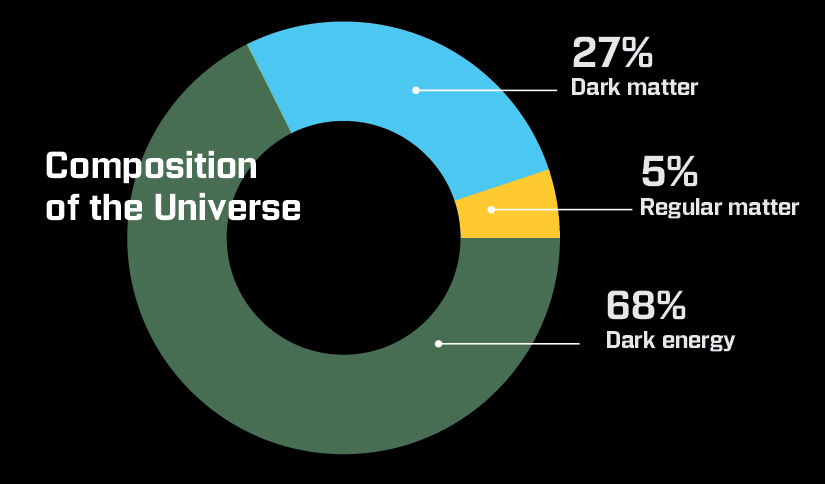
\includegraphics[scale=0.33]{figures/composition-of-universe.jpg}
    \end{figure}
\end{frame}

\begin{frame}{Open questions of the SM}
    \begin{itemize}
        \item The Standard Model is valid up to the Plank scale.
        \item The fundamental parameters of the Standard Model don’t reveal anything about these scales of energy
    \end{itemize}
    \begin{columns}
        \begin{column}{0.3\textwidth}
            \begin{figure}
                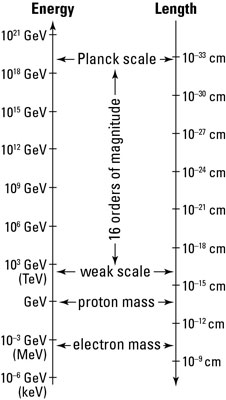
\includegraphics[scale=0.4]{figures/energy_scale.jpg}
            \end{figure}
        \end{column}
        \begin{column}{0.7\textwidth}
             \begin{itemize}
                \item Hierarchy problem:
                \begin{itemize}
                    \item Big gap in the energy scale
                    \item Weak scale and Plank scale: $\sim 10^{16}$
                    \item Weak force and gravational force: $\sim 10^{24}$
                \end{itemize}
                \item Higgs mass: $m^2_H = m^2_{bare} + \delta m^2_H$
                \begin{itemize}
                    \item $m_H \sim 125$~GeV
                    \item $\delta m^2_H = - \frac{|\lambda_{f}|^{2}}{8\pi}\Lambda_{UV}^{2}$ is quadratically divergent\\
                    At Plank scale $\Lambda_{UV}^{2} \sim 10^{19}$~GeV\\ $\Rightarrow$ $\delta m^2_H \sim 10^{38}$
                \end{itemize}
                \vspace{-0.5cm}
                \begin{figure}
                    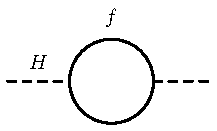
\includegraphics[scale=1.0]{figures/one-loop-correction-1.pdf}
                \end{figure}
            \end{itemize}
        \end{column}
    \end{columns}
    
\end{frame}

\begin{frame}{Open questions of the SM}
    \begin{itemize}
        \item Grand Unification Theory (GUT) expects:
        \begin{itemize}
            \item Electromagnetic, weak, and strong forces unify at GUT scale ($\sim 10^{16}$~GeV)
            \item Coupling constants $\alpha_{1}$, $\alpha_{2}$, and $\alpha_{3}$ converge
        \end{itemize}
    \end{itemize}
    \begin{columns}
        \begin{column}{0.6\textwidth}
            \vspace{-1cm}
            \begin{figure}
                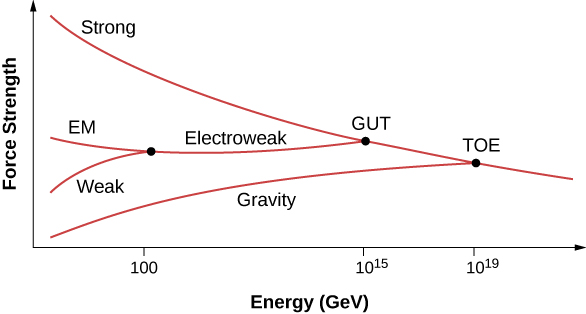
\includegraphics[scale=0.7]{figures/GUT.jpg}
            \end{figure}
            \begin{itemize}
                \item Theory of Everything (TOE): combines GUT and gravity (if possible)
            \end{itemize}
        \end{column}
        \begin{column}{0.4\textwidth}
            \begin{itemize}
                \item Coupling constants do not converge in the SM
            \end{itemize}
             \begin{figure}
                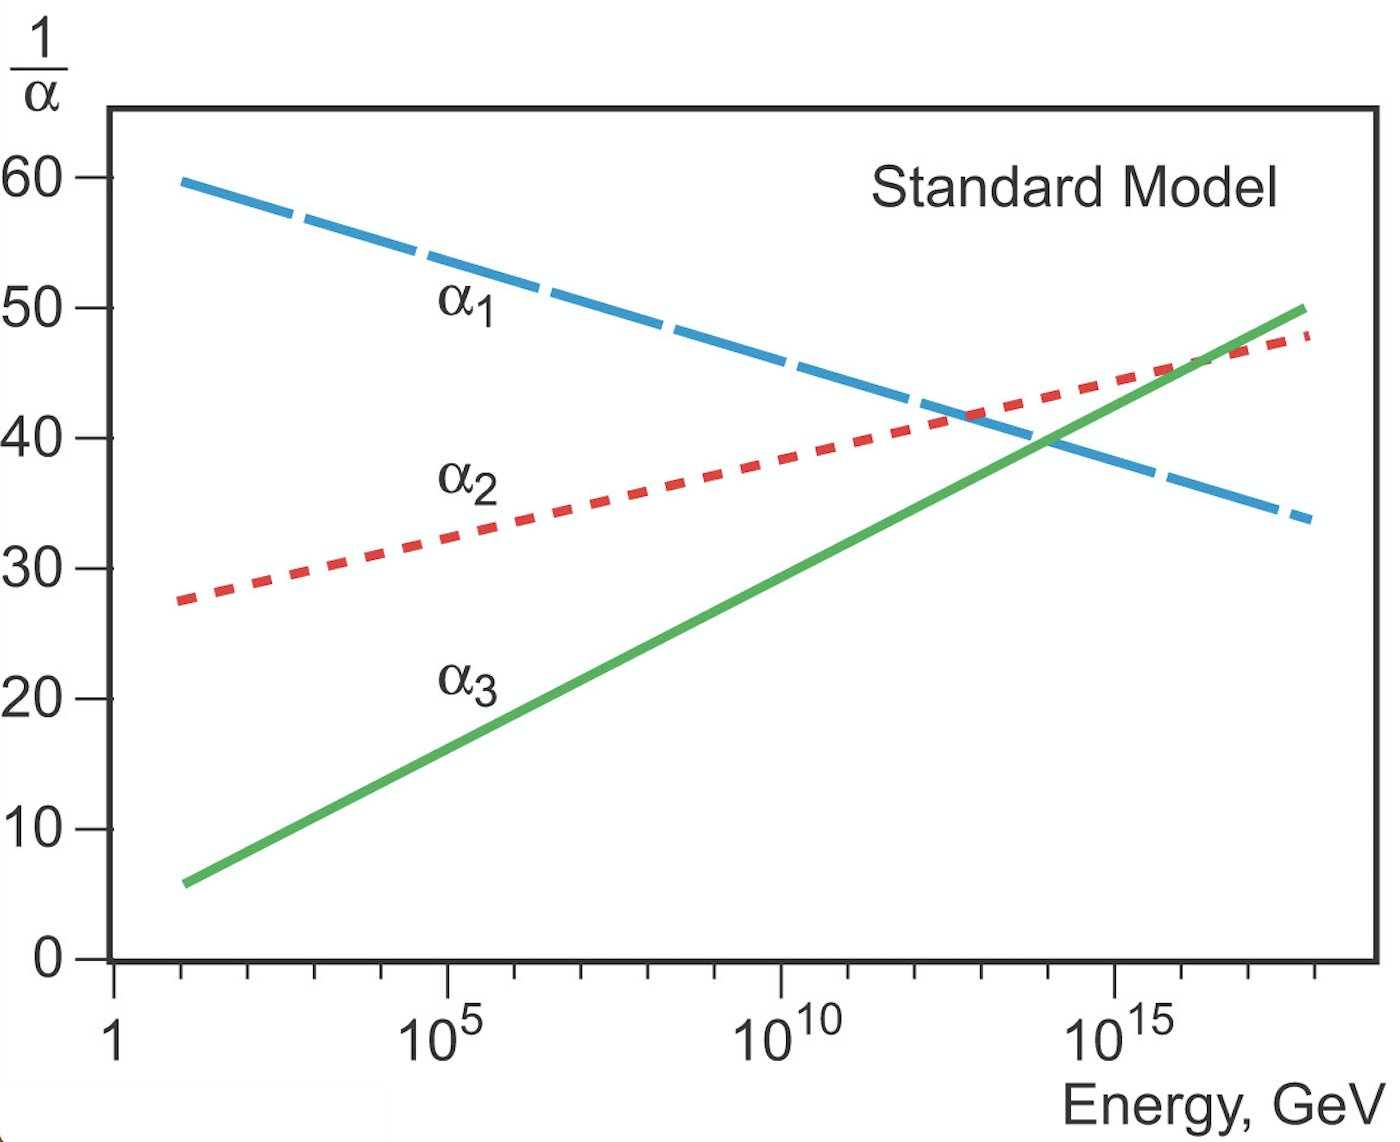
\includegraphics[scale=0.2]{figures/coupling_constants_sm.png}
            \end{figure}
        \end{column}
    \end{columns}
\end{frame}

{
\usebackgroundtemplate{%
    \tikz\node[opacity=0.2]{
        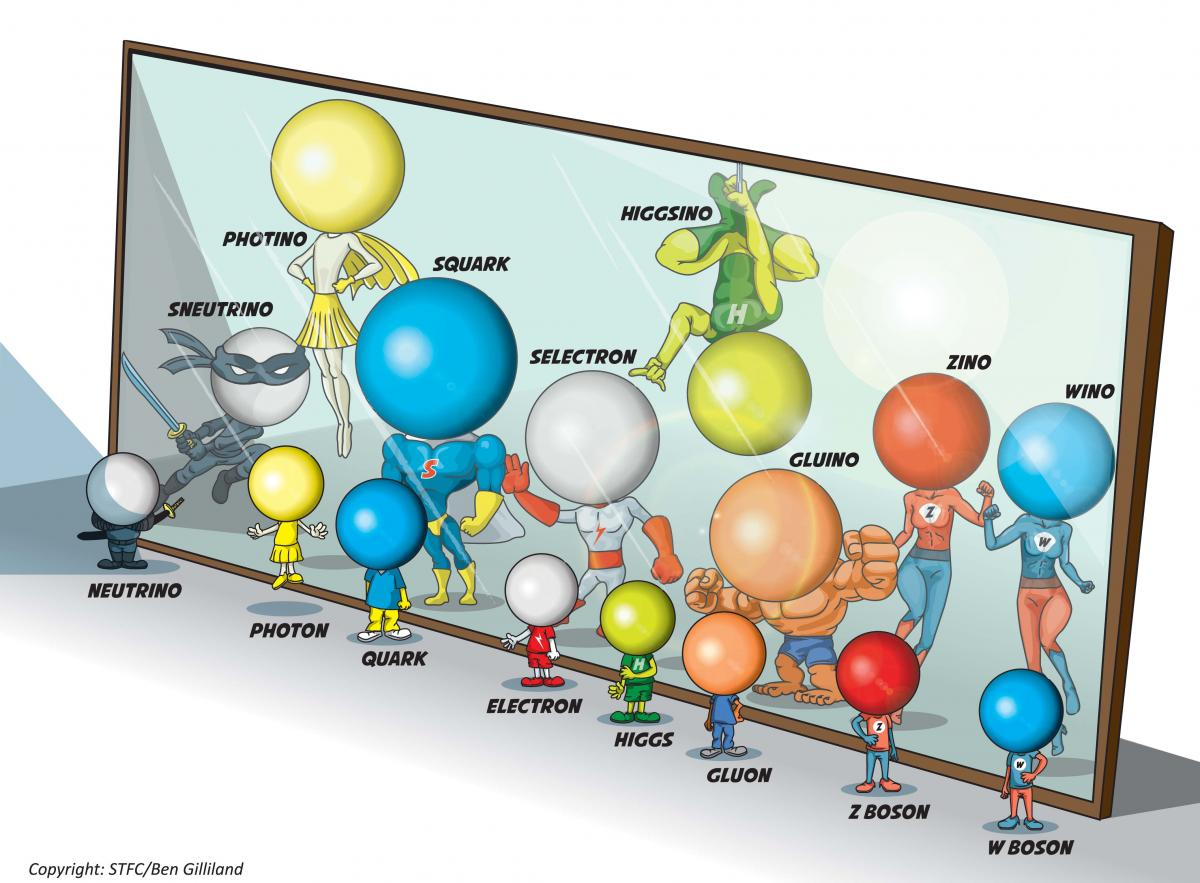
\includegraphics[height=\paperheight]{figures/susy-STFC.jpg}
    };
}    

\begin{frame}{Supersymmetry (SUSY)}
    \begin{itemize}
        \item Proposed by Wess and Zumino in early 1970
        \item Introduce supersymmetric partner particle to each SM particle
        \item Super particles have exactly the same quantum number as their SM partner particles except the spin differ by $\frac{1}{2}$
        \begin{center}
            Boson $\Leftarrow \Rightarrow$ Fermion
        \end{center}
    \end{itemize}
\end{frame}

\begin{frame}{Supersymmetry (SUSY)}
    \begin{itemize}
        \item SUSY answers:
        \begin{itemize}
            \item The hierarchy problem: opposite-sign loop corrections from SUSY particles\\
            \begin{columns}
                \begin{column}{0.2\textwidth}
                    \begin{figure}
                        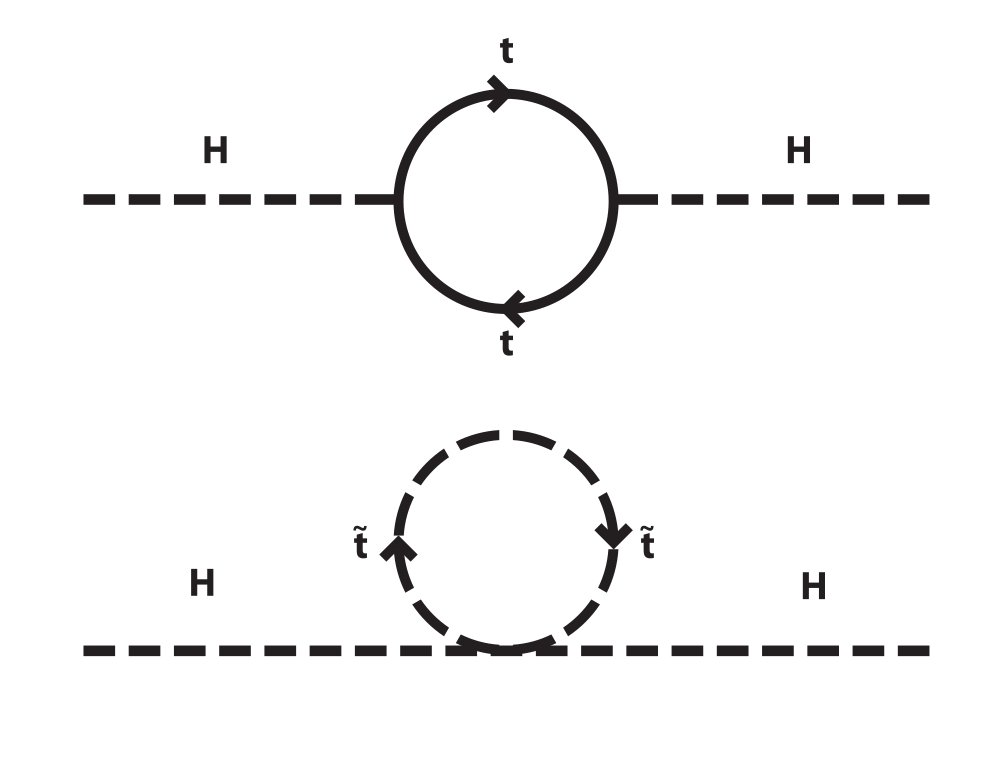
\includegraphics[scale=0.09]{figures/one-loop-correction.png}
                    \end{figure}
                \end{column}
                \begin{column}{0.2\textwidth}
                    \begin{align*}
                        & - \frac{|\lambda_{f}^{2}|}{8\pi^{2}} \Lambda_{UV}^{2}\\
                        & +\frac{\lambda_{S}}{16\pi^{2}} \Lambda_{UV}^{2} \times 2
                    \end{align*}
                \end{column}
            \end{columns}
            \item The candidate of Dark Matter: Lightest SUSY Particle (LSP)
            \item Coupling constants converge at GUT scale
            \begin{figure}
                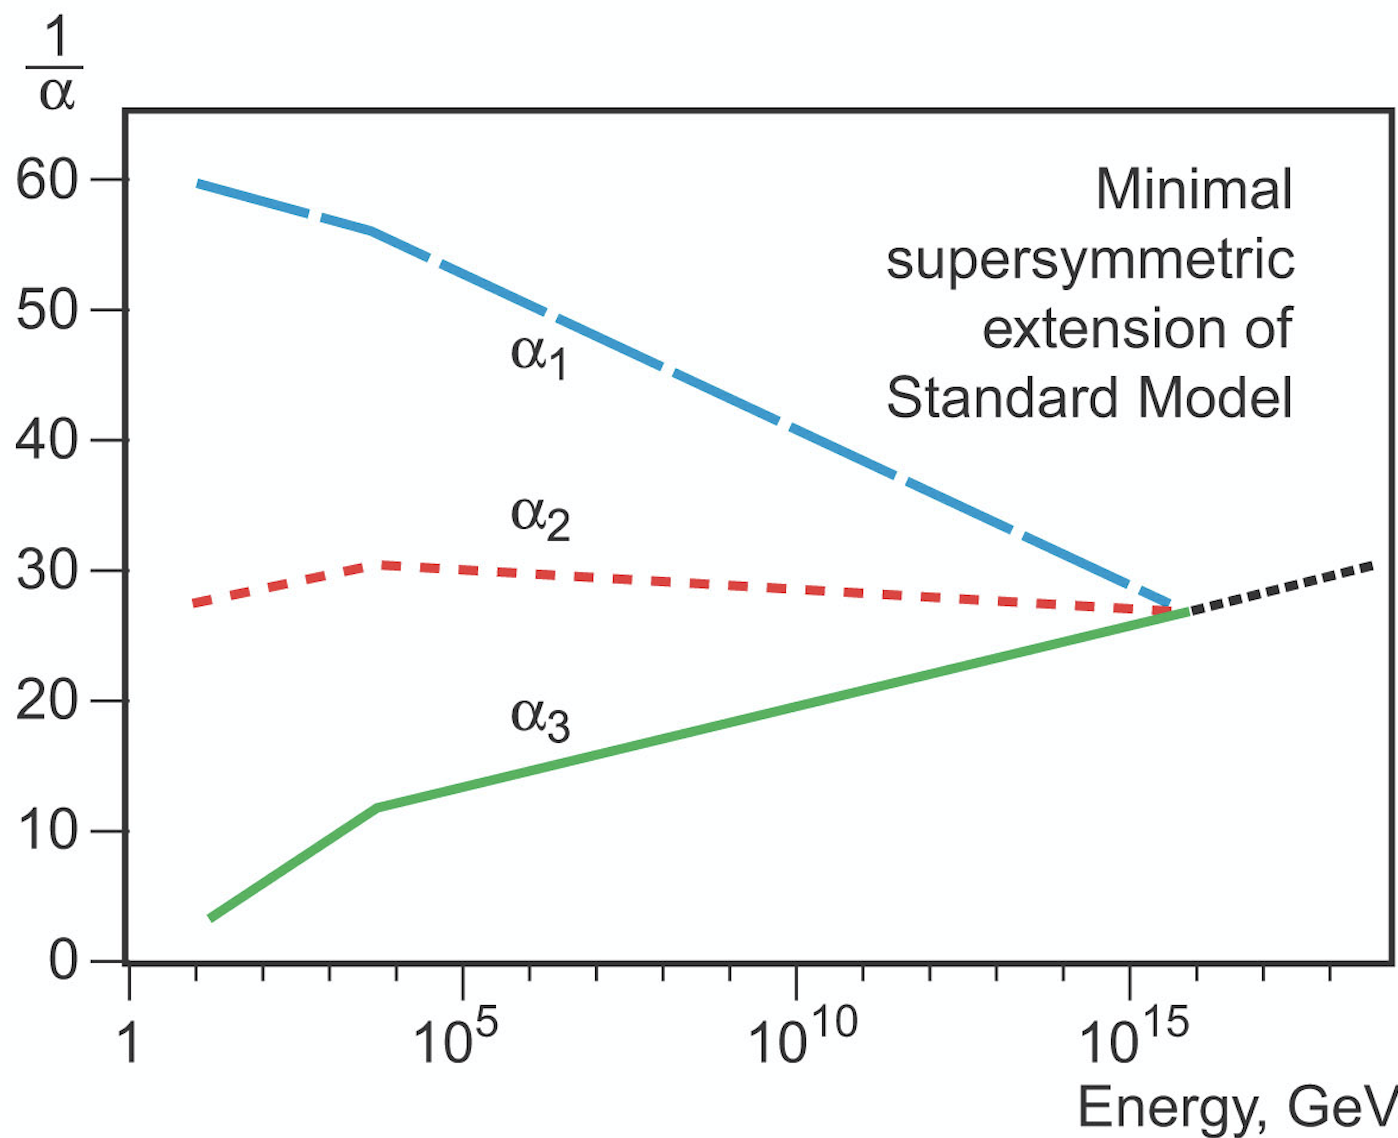
\includegraphics[scale=0.13]{figures/coupling_constants_susy.png}
            \end{figure}
            \item and more
        \end{itemize}
    \end{itemize}
\end{frame}
}

\section{Experimental Apparatus}
%\frame{\sectionpage}

{
\usebackgroundtemplate{
    \tikz\node[opacity=0.2]{
        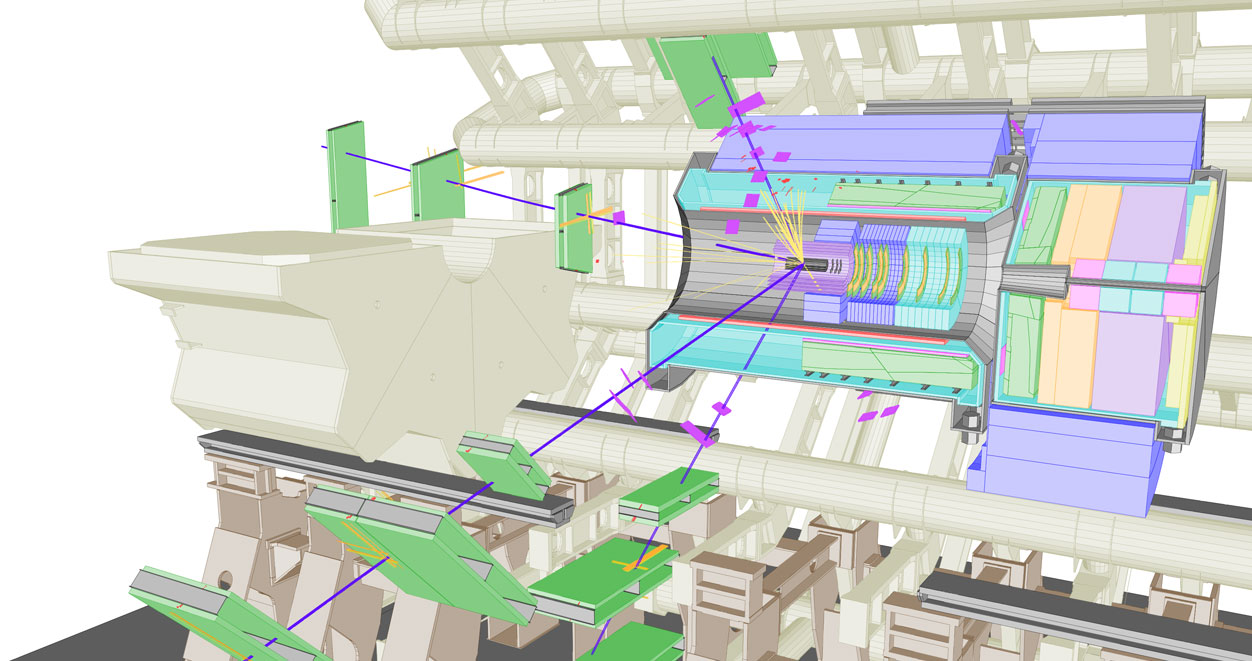
\includegraphics[scale=0.4]{figures/feature-1.jpg}
    };
}
\begin{frame}{Experimental Apparatus}
\end{frame}
}

\begin{frame}{The Large Hadron Collider (LHC)}
\end{frame}

\begin{frame}{ATLAS Detector}
\end{frame}


\section{Conclusion}
\frame{\sectionpage}

\begin{frame}{Conclusion}
    \begin{itemize}
        \item A slide
        \item with a title
        \item and some bullets
    \end{itemize}
\end{frame}

\end{document}
